\documentclass[11pt]{aghdpl}
% \documentclass[en,11pt]{aghdpl}  % praca w języku angielskim

% Lista wszystkich języków stanowiących języki pozycji bibliograficznych użytych w pracy.
% (Zgodnie z zasadami tworzenia bibliografii każda pozycja powinna zostać utworzona zgodnie z zasadami języka, w którym dana publikacja została napisana.)
\usepackage[english,polish]{babel}

% Użyj polskiego łamania wyrazów (zamiast domyślnego angielskiego).
\usepackage{polski}

\usepackage[utf8]{inputenc}

% dodatkowe pakiety

\usepackage{mathtools}
\usepackage{amsfonts}
\usepackage{amsmath}
\usepackage{amsthm}
\usepackage{algpseudocode}
\usepackage{algorithm}
\usepackage{listings}
\usepackage{color}
\usepackage{tikz}
\usepackage[T1]{fontenc}
%\usepackage[]{algorithm2e}

% --- < bibliografia > ---

\usepackage[
style=numeric,
sorting=none,
%
% Zastosuj styl wpisu bibliograficznego właściwy językowi publikacji.
language=autobib,
autolang=other,
% Zapisuj datę dostępu do strony WWW w formacie RRRR-MM-DD.
urldate=iso8601,
% Nie dodawaj numerów stron, na których występuje cytowanie.
backref=false,
% Podawaj ISBN.
isbn=true,
% Nie podawaj URL-i, o ile nie jest to konieczne.
url=false,
%
% Ustawienia związane z polskimi normami dla bibliografii.
maxbibnames=3,
% Jeżeli używamy BibTeXa:
backend=bibtex
]{biblatex}

\usepackage{csquotes}
% Ponieważ `csquotes` nie posiada polskiego stylu, można skorzystać z mocno zbliżonego stylu chorwackiego.
\DeclareQuoteAlias{croatian}{polish}

\addbibresource{bibliografia.bib}

% Nie wyświetlaj wybranych pól.
%\AtEveryBibitem{\clearfield{note}}


% ------------------------
% --- < listingi > ---

% Użyj czcionki kroju Courier.
\usepackage{courier}

\lstloadlanguages{TeX}

\lstset{
	literate={ą}{{\k{a}}}1
           {ć}{{\'c}}1
           {ę}{{\k{e}}}1
           {ó}{{\'o}}1
           {ń}{{\'n}}1
           {ł}{{\l{}}}1
           {ś}{{\'s}}1
           {ź}{{\'z}}1
           {ż}{{\.z}}1
           {Ą}{{\k{A}}}1
           {Ć}{{\'C}}1
           {Ę}{{\k{E}}}1
           {Ó}{{\'O}}1
           {Ń}{{\'N}}1
           {Ł}{{\L{}}}1
           {Ś}{{\'S}}1
           {Ź}{{\'Z}}1
           {Ż}{{\.Z}}1,
	basicstyle=\footnotesize\ttfamily,
}

% ------------------------

\AtBeginDocument{
	\renewcommand{\tablename}{Tabela}
	\renewcommand{\figurename}{Rys.}
}

% ------------------------
% --- < tabele > ---

\usepackage{array}
\usepackage{tabularx}
\usepackage{multirow}
\usepackage{booktabs}
\usepackage{makecell}
\usepackage[flushleft]{threeparttable}

% defines the X column to use m (\parbox[c]) instead of p (`parbox[t]`)
\newcolumntype{C}[1]{>{\hsize=#1\hsize\centering\arraybackslash}X}


%---------------------------------------------------------------------------

\author{Kamil Bienek}
\shortauthor{K. Bienek}

%\titlePL{Przygotowanie bardzo długiej i pasjonującej pracy dyplomowej w~systemie~\LaTeX}
%\titleEN{Preparation of a very long and fascinating bachelor or master thesis in \LaTeX}

\titlePL{Rozszerzenie kompilatora języka C/C++ do obsługi 8-bitowego procesora RISC}
\titleEN{C/C++ compiler extension for 8-bit RISC processors}


\shorttitlePL{Rozszerzenie kompilatora języka C/C++ do obsługi 8-bitowego procesora RISC} % skrócona wersja tytułu jeśli jest bardzo długi
\shorttitleEN{C/C++ compiler extension for 8-bit RISC processors}

\thesistype{Praca dyplomowa inżynierska}
%\thesistype{Master of Science Thesis}

\supervisor{dr. inż. Jakub Grela}
%\supervisor{Marcin Szpyrka PhD, DSc}

\degreeprogramme{Informatyka}
%\degreeprogramme{Computer Science}

\date{2021}

\department{Katedra Informatyki Stosowanej}
%\department{Department of Applied Computer Science}

\faculty{Wydział Elektrotechniki, Automatyki,\protect\\[-1mm] Informatyki i Inżynierii Biomedycznej}
%\faculty{Faculty of Electrical Engineering, Automatics, Computer Science and Biomedical Engineering}

\acknowledgements{Serdecznie dziękuję \dots tu ciąg dalszych podziękowań np. dla promotora, żony, sąsiada itp.}


\setlength{\cftsecnumwidth}{10mm}

%---------------------------------------------------------------------------
\setcounter{secnumdepth}{4}
\brokenpenalty=10000\relax


\lstdefinestyle{customasm}{
    belowcaptionskip=1\baselineskip,
    frame=single, 
    frameround=tttt,
    xleftmargin=\parindent,
    language=[x86masm]Assembler,
    basicstyle=\footnotesize\ttfamily,
    commentstyle=\itshape\color{green!60!black},
    keywordstyle=\color{blue!80!black},
    identifierstyle=\color{red!80!black},
    tabsize=4,
    numbers=left,
    numbersep=8pt,
    stepnumber=1,
    numberstyle=\tiny\color{black}, 
    columns = fullflexible,
}

\begin{document}

\titlepages

% Ponowne zdefiniowanie stylu `plain`, aby usunąć numer strony z pierwszej strony spisu treści i poszczególnych rozdziałów.
\fancypagestyle{plain}
{
	% Usuń nagłówek i stopkę
	\fancyhf{}
	% Usuń linie.
	\renewcommand{\headrulewidth}{0pt}
	\renewcommand{\footrulewidth}{0pt}
}

\setcounter{tocdepth}{2}
\tableofcontents
\clearpage

%\chapter{Przykłady elementów pracy dyplomowej}

\section{Liczba}

Pakiet \texttt{siunitx} zadba o to, by liczba została poprawnie sformatowana: \\
\begin{center}
	\num{1234567890.0987654321}
\end{center}


\section{Rysunek}

Pakiet \texttt{subcaption} pozwala na umieszczanie w podpisie rysunku odnośników do ,,podilustracji'': \\

\begin{figure}[h]
	\centering
	\begin{subfigure}{0.35\textwidth}
		\centering
		\framebox[2.0\width]{A}
		\subcaption{\label{subfigure_a}}
	\end{subfigure}
	\begin{subfigure}{0.35\textwidth}
		\centering
		\framebox[2.0\width]{B}
		\subcaption{\label{subfigure_b}}
	\end{subfigure}
	
	\caption{\label{fig:subcaption_example}Przykład użycia \texttt{\textbackslash subcaption}: \protect\subref{subfigure_a} litera A, \protect\subref{subfigure_b} litera B.}
\end{figure}

\section{Tabela}

Pakiet \texttt{threeparttable} umożliwia dodanie do tabeli adnotacji: \\

\begin{table}[h]
	\centering
	
	\begin{threeparttable}
		\caption{Przykład tabeli}
		\label{tab:table_example}
		
		\begin{tabularx}{0.6\textwidth}{C{1}}
			\toprule
			\thead{Nagłówek\tnote{a}} \\
			\midrule
			Tekst 1 \\
			Tekst 2 \\
			\bottomrule
		\end{tabularx}
		
		\begin{tablenotes}
			\footnotesize
			\item[a] Jakiś komentarz\textellipsis
		\end{tablenotes}
		
	\end{threeparttable}
\end{table}

\section{Wzory matematyczne}

Czasem zachodzi potrzeba wytłumaczenia znaczenia symboli użytych w równaniu. Można to zrobić z użyciem zdefiniowanego na potrzeby niniejszej klasy środowiska \texttt{eqwhere}.

\begin{equation}
E = mc^2
\end{equation}
gdzie
\begin{eqwhere}[2cm]
	\item[$m$] masa
	\item[$c$] prędkość światła w próżni
\end{eqwhere}

Odległość półpauzy od lewego marginesu należy dobrać pod kątem najdłuższego symbolu (bądź listy symboli) poprzez odpowiednie ustawienie parametru tego środowiska (domyślnie: 2 cm).

%\chapter{Wprowadzenie}
\label{cha:wprowadzenie}

\LaTeX~jest systemem składu umożliwiającym tworzenie dowolnego typu dokumentów (w~szczególności naukowych i technicznych) o wysokiej jakości typograficznej (\cite{Dil00}, \cite{Lam92}). Wysoka jakość składu jest niezależna od rozmiaru dokumentu -- zaczynając od krótkich listów do bardzo grubych książek. \LaTeX~automatyzuje wiele prac związanych ze składaniem dokumentów np.: referencje, cytowania, generowanie spisów (treśli, rysunków, symboli itp.) itd.

\LaTeX~jest zestawem instrukcji umożliwiających autorom skład i wydruk ich prac na najwyższym poziomie typograficznym. Do formatowania dokumentu \LaTeX~stosuje \TeX a (wymiawamy 'tech' -- greckie litery $\tau$, $\epsilon$, $\chi$). Korzystając z~systemu składu \LaTeX~mamy za zadanie przygotować jedynie tekst źródłowy, cały ciężar składania, formatowania dokumentu przejmuje na siebie system.

%---------------------------------------------------------------------------

\section{Cele pracy}
\label{sec:celePracy}


Celem poniższej pracy jest zapoznanie studentów z systemem \LaTeX~w zakresie umożliwiającym im samodzielne, profesjonalne złożenie pracy dyplomowej w systemie \LaTeX.

\subsection{Jakiś tytuł}

\subsubsection{Jakiś tytuł w subsubsection}


\subsection{Jakiś tytuł 2}

%---------------------------------------------------------------------------

\section{Zawartość pracy}
\label{sec:zawartoscPracy}

W rodziale~\ref{cha:pierwszyDokument} przedstawiono podstawowe informacje dotyczące struktury dokumentów w \LaTeX u. Alvis~\cite{Alvis2011} jest językiem 



















%\chapter{Pierwszy dokument}
\label{cha:pierwszyDokument}

W rozdziale tym przedstawiono podstawowe informacje dotyczące struktury prostych plików \LaTeX a. Omówiono również metody kompilacji plików z zastosowaniem programów \emph{latex} oraz \emph{pdflatex}.

%---------------------------------------------------------------------------

\section{Struktura dokumentu}
\label{sec:strukturaDokumentu}

Plik \LaTeX owy jest plikiem tekstowym, który oprócz tekstu zawiera polecenia formatujące ten tekst (analogicznie do języka HTML). Plik składa się z dwóch części:
\begin{enumerate}%[1)]
\item Preambuły -- określającej klasę dokumentu oraz zawierającej m.in. polecenia dołączającej dodatkowe pakiety;

\item Części głównej -- zawierającej zasadniczą treść dokumentu.
\end{enumerate}


\begin{lstlisting}
\documentclass[a4paper,12pt]{article}      % preambuła
\usepackage[polish]{babel}
\usepackage[utf8]{inputenc}
\usepackage[T1]{fontenc}
\usepackage{times}

\begin{document}                           % część główna

\section{Sztuczne życie}

% treść
% ąśężźćńłóĘŚĄŻŹĆŃÓŁ

\end{document}
\end{lstlisting}

Nie ma żadnych przeciwskazań do tworzenia dokumentów w~\LaTeX u w~języku polskim. Plik źródłowy jest zwykłym plikiem tekstowym i~do jego przygotowania można użyć dowolnego edytora tekstów, a~polskie znaki wprowadzać używając prawego klawisza \texttt{Alt}. Jeżeli po kompilacji dokumentu polskie znaki nie są wyświetlane poprawnie, to na 95\% źle określono sposób kodowania znaków (należy zmienić opcje wykorzystywanych pakietów).


%---------------------------------------------------------------------------

\section{Kompilacja}
\label{sec:kompilacja}


Załóżmy, że przygotowany przez nas dokument zapisany jest w pliku \texttt{test.tex}. Kolejno wykonane poniższe polecenia (pod warunkiem, że w pierwszym przypadku nie wykryto błędów i kompilacja zakończyła się sukcesem) pozwalają uzyskać nasz dokument w formacie pdf:
\begin{lstlisting}
latex test.tex
dvips test.dvi -o test.ps
ps2pdf test.ps
\end{lstlisting}
%
lub za pomocą PDF\LaTeX:
\begin{lstlisting}
pdflatex test.tex
\end{lstlisting}

Przy pierwszej kompilacji po zmiane tekstu, dodaniu nowych etykiet itp., \LaTeX~tworzy sobie spis rozdziałów, obrazków, tabel itp., a dopiero przy następnej kompilacji korzysta z tych informacji.

W pierwszym przypadku rysunki powinny być przygotowane w~formacie eps, a~w~drugim w~formacie pdf. Ponadto, jeżeli używamy polecenia \texttt{pdflatex test.tex} można wstawiać grafikę bitową (np. w formacie jpg).



%---------------------------------------------------------------------------

\section{Narzędzia}
\label{sec:narzedzia}


Do przygotowania pliku źródłowego może zostać wykorzystany dowolny edytor tekstowy. Niektóre edytory, np. GEdit, mają wbudowane moduły ułatwiające składanie tekstów w LaTeXu (kolorowanie składni, skrypty kompilacji, itp.).

Jednym z bardziej znanych środowisk do składania dokumentów  \LaTeX a jest {\em TeXstudio}, oferujące kompletne środowisko pracy. Zobacz: \url{http://www.texstudio.org}


Bardzo dobrym środowiskiem jest również edytor gEdit z wtyczką obsługującą \LaTeX a. Jest to standardowy edytor środowiska Gnome. Po instalacji wtyczki obsługującej \LaTeX~ zamienia się w wygodne i szybkie środowisko pracy.

\textbf{Dla testu łamania stron powtórzenia powyższego tekstu.}


Do przygotowania pliku źródłowego może zostać wykorzystany dowolny edytor tekstowy. Niektóre edytory, np. GEdit, mają wbudowane moduły ułatwiające składanie tekstów w LaTeXu (kolorowanie składni, skrypty kompilacji, itp.).
Jednym z bardziej znanych środowisk do składania dokumentów  \LaTeX a jest {\em TeXstudio}, oferujące kompletne środowisko pracy. Zobacz: \url{http://www.texstudio.org}
Bardzo dobrym środowiskiem jest również edytor gEdit z wtyczką obsługującą \LaTeX a. Jest to standardowy edytor środowiska Gnome. Po instalacji wtyczki obsługującej \LaTeX~ zamienia się w wygodne i szybkie środowisko pracy.
Po instalacji wtyczki obsługującej \LaTeX~ zamienia się w wygodne i szybkie środowisko pracy.

Do przygotowania pliku źródłowego może zostać wykorzystany dowolny edytor tekstowy. Niektóre edytory, np. GEdit, mają wbudowane moduły ułatwiające składanie tekstów w LaTeXu (kolorowanie składni, skrypty kompilacji, itp. itd. itp.).
Jednym z bardziej znanych środowisk do składania dokumentów  \LaTeX a jest {\em TeXstudio}, oferujące kompletne środowisko pracy. Zobacz: \url{http://www.texstudio.org}
Bardzo dobrym środowiskiem jest również edytor gEdit z wtyczką obsługującą \LaTeX a. Jest to standardowy edytor środowiska Gnome. Po instalacji wtyczki obsługującej \LaTeX~ zamienia się w wygodne i szybkie środowisko pracy.

Do przygotowania pliku źródłowego może zostać wykorzystany dowolny edytor tekstowy. Niektóre edytory, np. GEdit, mają wbudowane moduły ułatwiające składanie tekstów w LaTeXu (kolorowanie składni, skrypty kompilacji, itp.).
Jednym z bardziej znanych środowisk do składania dokumentów  \LaTeX a jest {\em TeXstudio}, oferujące kompletne środowisko pracy. Zobacz: \url{http://www.texstudio.org}
Bardzo dobrym środowiskiem jest również edytor gEdit z wtyczką obsługującą \LaTeX a. Jest to standardowy edytor środowiska Gnome. Po instalacji wtyczki obsługującej \LaTeX~ zamienia się w wygodne i szybkie środowisko pracy.

%---------------------------------------------------------------------------

\section{Przygotowanie dokumentu}
\label{sec:przygotowanieDokumentu}

Plik źródłowy \LaTeX a jest zwykłym plikiem tekstowym. Przygotowując plik
źródłowy warto wiedzieć o kilku szczegółach:

\begin{itemize}
\item
Poszczególne słowa oddzielamy spacjami, przy czym ilość spacji nie ma znaczenia.
Po kompilacji wielokrotne spacje i tak będą wyglądały jak pojedyncza spacja.
Aby uzyskać {\em twardą spację}, zamiast znaku spacji należy użyć znaku {\em
tyldy}.

\item
Znakiem końca akapitu jest pusta linia (ilość pusty linii nie ma znaczenia), a
nie znaki przejścia do nowej linii.

\item
\LaTeX~sam formatuje tekst. \textbf{Nie starajmy się go poprawiać}, chyba, że
naprawdę wiemy co robimy.
\end{itemize} 



%\chapter{Testy}

\section{Test URL-a}

Wejdź na stronę \url{https://www.google.pl/} i wpisz szukane zdanie.

\clearpage

\section{Test dzielenia wdów}

Lorem ipsum dolor sit amet, ex est alia dolorem commune. Duo modo errem no. Ea harum doming atomorum mei. Consul animal malorum cu qui, sumo dicta graece an est, vim ei clita regione.

Vel eu quando doming fastidii, mei graeco indoctum an, legere theophrastus in pro. Te mei probatus eleifend interpretaris. Est no autem liber vituperatoribus, cu mea dicam constituto. Ea laudem tritani consectetuer sit, sanctus patrioque expetendis vix in. Duo id fugit adversarium signiferumque, an quot modus molestiae qui.

Ut paulo definiebas pro. Mea an quod esse. Et atomorum facilisis moderatius sit. Graeco iudicabit forensibus in vel. Eam cu lorem aeterno offendit, cu vix nulla congue posidonium. Vel lucilius evertitur vituperata no.

Mea eu graecis prodesset. Et tota eius nec. Ei etiam oratio has, vel ei homero eripuit invenire. Sed ex errem intellegebat, sea et elitr intellegat constituto. Nostro voluptua accusamus eos in, ei sale admodum has. Vim ne consetetur reformidans, ad has malis recusabo persequeris, per etiam virtute invenire in.

Te nihil eruditi eam, sit aperiam accusam mediocritatem at. Nec ne nonumy dictas disputationi, vis ridens sadipscing ex. Harum euripidis ex vix, at consetetur instructior signiferumque mel, at mei elitr honestatis. Id sit congue vituperata. Temporibus eloquentiam no eum.

Pro id esse phaedrum, nostro iudicabit eos ut. Sit ea aperiam alienum, harum audiam voluptua cu usu. Iudico invenire te vel, id suscipit disputando pri. Ut sumo expetenda mea.

Cum at idque nullam aperiam, vis ex aeque ponderum luptatum. Vix soluta graeco dissentiet ut, ut est reque periculis similique, ut dicta dicant repudiare sea. Ne dolor legendos signiferumque ius, at eirmod convenire qui. Suas numquam conceptam mei ex. Autem homero eos et, sea dicta alienum iudicabit ut.

Ea duo consulatu vulputate, id elit perpetua cum. His ei aeque saepe audiam. Prompta laoreet facilisi ne sed, per hinc consetetur te, oratio fuisset ullamcorper mel at. Quis suscipiantur ne nec, agam efficiendi usu in.

Vis eu iuvaret singulis appellantur, usu ex saepe omittantur. Sed possit mnesarchum at, usu illum choro oratio in, et debet dolor vix. Mel aperiri suscipiantur ne, te per illum fuisset, lorem pericula mei ad. Pri id tale lucilius dissentiet, id sea sonet expetenda. Agam sensibus persequeris sed no, eum at tamquam sanctus.

Omnis exerci soleat ut vis. Rebum vidisse sea ex. Ius animal gubergren efficiantur ad, mollis probatus nec ut. Meis platonem ex vel, ut qui tale tritani equidem. Vide meis fuisset mel at, nam an assum delenit gubergren. No illum reprimique vim, te augue nullam per, ludus dicant suscipiantur ne sed.

An pri mediocrem deseruisse, ad sumo audire dissentiet sit. Sit ea civibus lobortis. Etiam ceteros commune ei vis. Pro ei equidem vivendo. Quo ne prima periculis omittantur, ex rebum veritus sit, ei dolor maiestatis mea.

\subsection{Lorem ipsum}

Et mel munere quodsi sapientem. Essent legimus ne pro. Est ornatus definiebas et. No habemus docendi ius, purto sapientem mei at. Tamquam vivendo necessitatibus has at, no habemus praesent nec. No quo modus iudicabit scriptorem. Modus intellegebat ea vim. Cu ius lorem regione offendit, ne accusata sensibus vituperatoribus quo. Sit ut iuvaret indoctum. Ut mea sale justo. Sapientem definitionem ius eu, at sea quem doming. Facete conclusionemque ut nec, vix at duis eius. Eos quot consequuntur et, ornatus liberavisse ne mei.

Per an dicam commodo tractatos, usu in timeam numquam tacimates. Case delectus eu sea, usu audiam eleifend tincidunt id, nec at decore discere mentitum. Ut elit veri eloquentiam his, ceteros tractatos ea has. Duo impetus scribentur et, eu quo errem everti, ad recusabo consulatu ius. Fastidii comprehensam pri ea, ex duo augue quando denique. Eos aeterno deserunt sententiae cu, ius quas tation patrioque ex.

Id autem scripta explicari nec, congue quidam possit te sit. Et usu ipsum bonorum graecis, ferri verear deterruisset eum cu. Purto porro accommodare cu vim. Cum ei tritani pertinacia voluptaria.

\chapter{Wstęp}
\section{Cele pracy}
\subsection{Rozszerzenie kompilatora}
\subsection{Wizualizacja}
\section{Zawartość pracy}

\chapter{Analiza literatury?}

\chapter{Procesor}
\section{Architektura RISC}
\section{Rejestry}
\section{Instrukcje}
\section{Format instrukcji}

\chapter{Kompilator}
\section{Struktura}
\section{AVR}
\subsection{AVR-gcc}
\subsection{instrukcje?}
\section{MOS 6502}
\subsection{Instrukcje}

\chapter{Konwerter}
\section{Struktura}
\section{Działanie}

\chapter{Implementacja operacji arytmetycznych}
\section{Operacje na liczbach całkowitych}
\subsection{Dodawanie dwóch liczb ośmiobitowych}
\iffalse
\begin{algorithm}
\caption{An algorithm with caption}\label{alg:cap}
\begin{algorithmic}
\Require $a \geq 0, b \geq 0$
\Ensure $c = a + b$
\State LIL [B]
\State LIH [B]
\State MMA
\State LDA
\State MBA
\State LIL [A]
\State LIH [A]
\State MMA
\State LDA
\State CLC
\State ADL
\State ADH
\State LIL [C]
\State LIH [C]
\State MMA
\State MAC
\State STA

\end{algorithmic}
\end{algorithm}
\fi
\subsection{Odejmowanie dwóch liczb ośmiobitowych}
\iffalse
\begin{algorithm}
\caption{An algorithm with caption}\label{alg:cap}
\begin{algorithmic}
\Require $a \geq 0, b \geq 0$
\Ensure $c = a - b$
\State LIL [B]
\State LIH [B]
\State MMA
\State LDA
\State NOT
\State MAC
\State MBA
\State LIL [A]
\State LIH [A]
\State MMA
\State LDA
\State SEC
\State ADL
\State ADH
\State LIL [C]
\State LIH [C]
\State MMA
\State MAC
\State STA

\end{algorithmic}
\end{algorithm}
\fi
\subsection{Mnożenie dwóch liczb ośmiobitowych}
\iffalse
\begin{algorithm}
\caption{An algorithm with caption}\label{alg:cap}
\begin{algorithmic}
\Require $a \geq 0, b \geq 0$
\Ensure $c = a * b$

\State LIL [B]
\State LIH [B]
\State MMA
\State LDA
\State SHR
\State LIL 0x0
\State LIH 0x0
\State MBA
\State ADL
\State ADH
\State LIX mul
\State MMA
\State JNE
\State LIL ?
\State LIH ?
\State MMA
\State LDA
\State CLC
\State ADL
\State ADH
\State MAC
\State STA
\State 
\State 
\State 
\State 
\State 

\State ...
\State mul:
\State LIL ?
\State LIH ?
\State MMA
\State LDA
\State 
\State 
\State 
\State 
\State 
\State 
\State 
\State 

\end{algorithmic}
\end{algorithm}
\fi
\section{Liczby zmiennopozycyjne w standardzie IEEE-754}

\section{Dodawanie liczb zmiennopozycyjnych}
\subsection{Pseudokod}
\begin{algorithm}

\caption{IEEE-754 addition}
\iffalse
\KwData{ a - normalized float , b - normalized float}
\KwResult {c = a + b}
\fi
\begin{algorithmic}[1]
\Require a - normalized float \\
		 b - normalized float
\Ensure c = a + b
\State $NOP$
\State $NOP$
\State $NOP$
\State $NOP$
\State $NOP$
\State $NOP$
\State $NOP$
\State $NOP$
\State $NOP$
\State $NOP$
\State $NOP$
\algstore{myalg}
\end{algorithmic}
\end{algorithm}

\begin{algorithm}
\begin{algorithmic}[1]
\algrestore{myalg}
\State $NOP$
\State $NOP$
\State $NOP$
\State $NOP$
\State $NOP$
\State $NOP$
\State $NOP$
\State $NOP$
\State $NOP$
\State $NOP$
\State $NOP$


\iffalse
\If {a = 0}{
	c ← b
}

\If {b = 0}{
	c ← a
}


asgn $\leftarrow$ a[31]

aexp ← a[30..23]

aman ← a[22..0]

bsgn ← b[31]

bexp ← b[30..23]

bman ← b[22..0]

\If {aexp = 255}{
	\If {a = NaN}{
		c ← NaN
	}
	\If {a = Inf}{
		\If {bexp = 255}{
			\If {b = NaN}{
				c ← NaN
			}
			\If {b = Inf}{
				\eIf {asgn = bsgn}{
					c ← a
				}{
					c ← NaN
				}
			}
		}
	}
}
\fi
\end{algorithmic}
\end{algorithm}

\cleardoublepage
\subsection{UML}

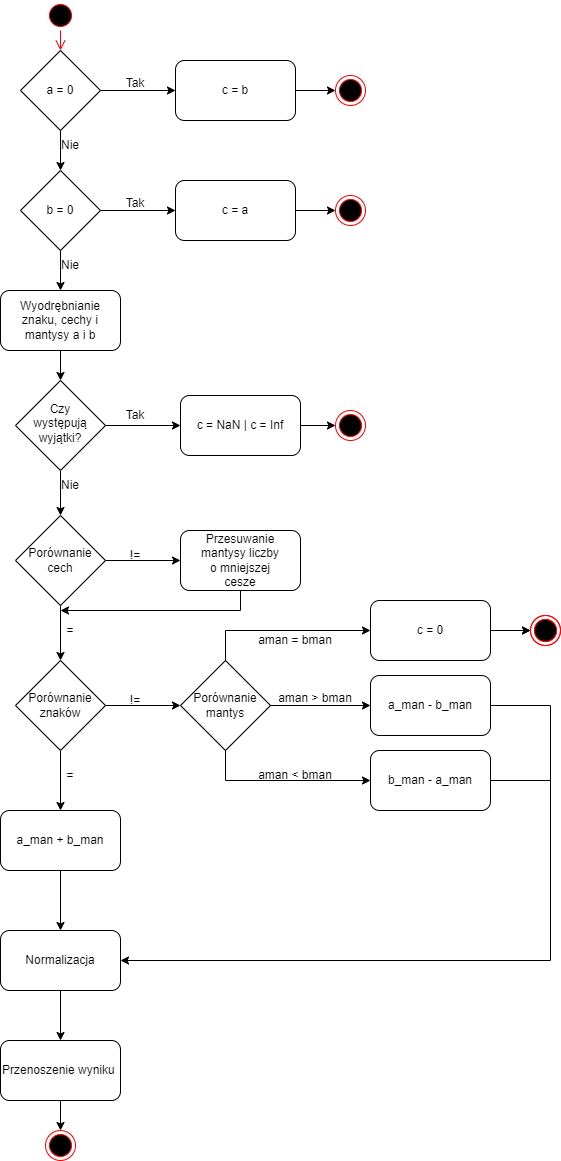
\includegraphics[scale=0.55]{addition_uml}

\begin{lstlisting}[style=customasm, caption={Dodawanie liczb zmiennopozycyjnych}, label=float_addition]
addf: LIX compare_exp
        MMA
        JMP
cmp:       LIL [B]+1
        LIH [B]+1
MMA
LDA
SHL
LIL 0x0
LIH 0x0
MBA
ADL
ADH
MAC
MBA
LIL [B]
LIH [B]
MMA
LDA
SHL
MAC
CLC
OR
LIL [expB]
LIH [expB]
MMA
MAC
STA

LIL [A]+1
LIH [A]+1
MMA
LDA
SHL
LIL 0x0
LIH 0x0
MBA
ADL
ADH
MAC
MBA
LIL [A]
LIH [A]
MMA
LDA
SHL
MAC
CLC
OR
LIL [expA]
LIH [expA]
MMA
MAC
STA

LIL [expB]
LIH [expB]
MMA
LDA
MBA
MAC

XOR
LIX not_equal
MMA
JNE
LIX equal
MMA
JMP

not_equal:
LIL ST
LIH ST
MMA
MAC
STA
LIL ST-1
LIH ST-1
MMA
LIL 0x0
LIH 0x0
OR
MAC
STA

loop:
LIL ST
LIH ST
MMA
LDA
CLC
SHL
MAC
STA
LIL 0x0
LIH 0x0
MBA
ADL
ADH
LIX check
MMA
JNE
LIL ST-1
LIH ST-1
MMA
LDA
SHL
MAC
STA
LIX loop
MMA
JMP
HLT

check:
LIL ST-1
LIH ST-1
MMA
LDA
SHL
LIL 0x0
LIH 0x0
MBA
ADL
ADH
LIX higherB
MMA
JNE
LIX lowerB
MMA
JMP

higherB:
LIL [expA]
LIH [expA]
MMA
LDA
NOT
MAC
MBA
LIL [expB]
LIH [expB]
MMA
LDA
SEC
ADL
ADH
LIL [exp]
LIH [exp]
MMA
MAC
STA
// przenoszenie
LIL [A]+1
LIH [A]+1
MMA
LDA
MBA
LIL 0xF
LIH 0x7
AND
LIL [manA]
LIH [manA]
MMA
MAC
STA
LIL 0x0
LIH 0x0
MBA
LIL [A]+2
LIH [A]+2
MMA
LDA
OR
LIL [manA]+1
LIH [manA]+1
MMA
MAC
STA
LIL [A]+3
LIH [A]+3
MMA
LDA
OR
LIL [manA]+2
LIH [manA]+2
MMA
MAC
STA

higherBloop:
LIL [manA]
LIH [manA]
MMA
LDA
SHR
MAC
STA
LIL [manA]+1
LIH [manA]+1
MMA
LDA
SHR
MAC
STA
LIL [manA]+2
LIH [manA]+2
MMA
LDA
SHR
MAC
STA

LIL [exp]
LIH [exp]
MMA
LDA
MBA
LIL 0x1
LIH 0x0
NOT
MAC
SEC
ADL
ADH
MAC
STA
LIX higherBloop
MMA
JNE
LIX equals
MMA
JMP

lowerB:
LIL [expB]
LIH [expB]
MMA
LDA
NOT
MAC
MBA
LIL [expA]
LIH [expA]
MMA
LDA
SEC
ADL
ADH
LIL [exp]
LIH [exp]
MMA
MAC
STA
// przenoszenie
LIL [B]+1
LIH [B]+1
MMA
LDA
MBA
LIL 0xF
LIH 0x7
AND
LIL [manB]
LIH [manB]
MMA
MAC
STA
LIL 0x0
LIH 0x0
MBA
LIL [B]+2
LIH [B]+2
MMA
LDA
OR
LIL [manB]+1
LIH [manB]+1
MMA
MAC
STA
LIL [B]+3
LIH [B]+3
MMA
LDA
OR
LIL [manB]+2
LIH [manB]+2
MMA
MAC
STA

lowerBloop:
LIL [manB]
LIH [manB]
MMA
LDA
SHR
MAC
STA
LIL [manB]+1
LIH [manB]+1
MMA
LDA
SHR
MAC
STA
LIL [manB]+2
LIH [manB]+2
MMA
LDA
SHR
MAC
STA

LIL [exp]
LIH [exp]
MMA
LDA
MBA
LIL 0x1
LIH 0x0
NOT
MAC
SEC
ADL
ADH
MAC
STA
LIX lowerBloop
MMA
JNE
LIX equals
MMA
JMP

equal:
//---dodawanie mantys
LIL [B] + 3
LIL [B] + 3
MMA
LDA
MBA
LIL [A] + 3
LIH [A] + 3
MMA
LDA
CLC
ADL
ADH
LIL [C] + 3
LIH [C] + 3
MMA
MAC
STA

LIL [B] + 2
LIL [B] + 2
MMA
LDA
MBA
LIL [A] + 2
LIH [A] + 2
MMA
LDA
ADL
ADH
LIL [C] + 2
LIH [C] + 2
MMA
MAC
STA

LIL [B] + 1
LIL [B] + 1
MMA
LDA
MBA
LIL 0xF
LIH 0x7
AND
LIL [C] + 1
LIH [C] + 1
MMA
MAC
STA
LIL [A] + 1
LIH [A] + 1
MMA
LDA
MBA
LIL 0xF
LIH 0x7
AND
LIL [C] + 1
LIH [C] + 1
MMA
LDA
MBA
MAC
ADL
ADH
LIL 0xF
LIH 0x7
MBA
CLC
MAC
AND
MAC
STA
//---koniec dodawanie mantys

LIL [A] + 1
LIH [A] + 1
MMA
LDA
MBA
LIL 0x0
LIH 0x8
AND
LIL [C] + 1
LIH [C] + 1
MMA
LDA
MBA
MAC
OR
MAC
STA

LIL [A]
LIH [A]
MMA
LDA
MBA
LIL [C]
LIH [C]
MMA
LIL 0x0
LIH 0x0
OR
MAC
STA

HLT


equalall:
//---dodawanie mantys
LIL [manB] + 2
LIL [manB] + 2
MMA
LDA
MBA
LIL [manA] + 2
LIH [manA] + 2
MMA
LDA
CLC
ADL
ADH
LIL [C] + 3
LIH [C] + 3
MMA
MAC
STA

LIL [manB] + 1
LIL [manB] + 1
MMA
LDA
MBA
LIL [manA] + 1
LIH [manA] + 1
MMA
LDA
ADL
ADH
LIL [C] + 2
LIH [C] + 2
MMA
MAC
STA

LIL [manB]
LIL [manB]
MMA
LDA
MBA
LIL [manA]
LIH [manA]
MMA
LDA
ADL
ADH
LIL [C] + 1
LIH [C] + 1
MMA
MAC
STA
//---koniec dodawanie mantys

LIL [B] + 1
LIH [B] + 1
MMA
LDA
MBA
LIL 0x0
LIH 0x8
AND
LIL [C] + 1
LIH [C] + 1
MMA
LDA
MBA
MAC
OR
MAC
STA

LIL [B]
LIH [B]
MMA
LDA
MBA
LIL [C]
LIH [C]
MMA
LIL 0x0
LIH 0x0
OR
MAC
STA

HLT
\end{lstlisting}





\chapter{Wizualizacja}
\section{Symulator}

\chapter{Przykłady}
\section{Przykład A}
\section{Przykład B}
\section{Przykład C}


\chapter{Podsumowanie}

% itd.
% \appendix
% \include{dodatekA}
% \include{dodatekB}
% itd.



\printbibliography

\end{document}
